\chapter{神经符号框架的架构设计与实现}
\section{引言}
本章对神经符号框架的架构进行详细的介绍,包括流水线总体架构、视觉场景理解、语义解析、迭代反馈和规则修正、规则蒸馏、ASP推理等模块的设计和实现。
框架的目标如下:
\begin{enumerate}[label=(\arabic*),itemsep=0pt,parsep=0pt]
\item 增强VQA系统在复杂空间关系推理方面的能力。
\item 使用Dspy来完成对LLM的提示、优化,以降低神经符号方法的开发难度,并增强其可扩展性。
\item 
\end{enumerate}
\section{框架总体架构}
框架的总体架构如图\ref{fig:pipeline}所示。其中,LLM在整个框架中的作用有以下两点:
\begin{enumerate}[label=(\arabic*),itemsep=0pt,parsep=0pt]
    \item 在语义解析模块中,LLM对自然语言问题进行语义解析,将问题以ASP的形式表示出来,以便后续
输入到迭代反馈模块中进行修正。
    \item 在迭代反馈模块中,LLM对ASP表示进行多次迭代优化,其中包括解析错误、基础化错误等。每一轮迭代都将
根据上一轮的错误信息进行针对性的修正。
    \item 在规则蒸馏中,LLM结合ASP知识库中的先验知识,对迭代反馈修正后ASP规则进行进一步补全,为Clingo求解器
推理提供更全面的知识。
    \item 在求解结果翻译中,LLM对Clingo求解器输出的以ASP表示的结果进行翻译,使其以自然语言形式,针对提出的问题
进行作答。
添加规则,对规则进行一致性检查以及整合错误信息的反馈。
\end{enumerate}
\begin{figure}
    \centering
    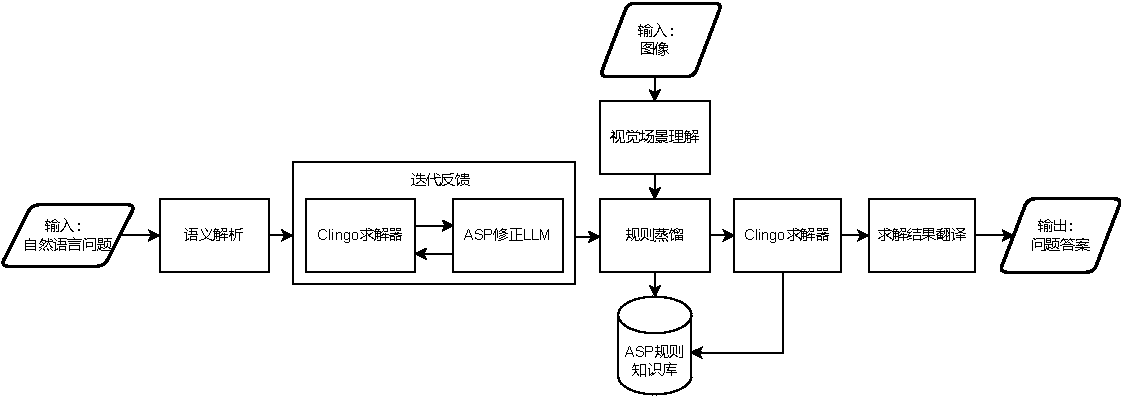
\includegraphics[width=\textwidth]{figures/pipeline-crop.pdf}
    \caption{面向空间推理领域的神经符号框架示意图}
    \label{fig:pipeline}
\end{figure}
本文在语义解析模块和迭代反馈模块中,分别采用不同的LLM,各自进行微调,以更好地满足不同任务的需求。
\section{视觉场景理解}
视觉场景理解是本文所设计流水线中的核心模块,其目标是从输入图像中提取结构化信息,包括物体的属性(如形状、颜色、大小等)、位置信息以及物体间的空间关系。这些信息将被进一步转换为ASP的形式,为后续基于逻辑推理的语义解析与问答模块提供形式化的知识基础。

本章主要围绕以下四个方面展开详细阐述:目标检测、空间位置提取、空间关系提取以及场景图生成。最后,本文给出一个完整的视觉场景理解演示案例,并讨论在实现过程中遇到的关键技术挑战及相应解决方案。
\subsection{目标检测}
目标检测是视觉场景理解的最基础的任务,其目标是从图像中识别出所有相关物体,并标注其边界框、类别和属性。本文选择GLIP模型作为目标检测的实现工具,原因在于
其独特的语言-视觉预训练特性。基于大规模的图文对数据,GLIP进行大量预训练,能够根据自然语言描述(如“红色立方体”)直接定位图像中的对应物体。
这种能力特别适合VQA任务,使问题中的语言信息与图像内容高效对齐成为可能。

目标检测是视觉场景理解的基础任务,其任务是从输入图像中识别出所有相关物体,
并为每个物体确定其边界框、类别和相关属性。本文采用了GLIP模型作为目标检测的核心工具,其主要优势体现在:
\begin{enumerate}[label=(\arabic*),itemsep=0pt,parsep=0pt] 
\item \textbf{语言-视觉预训练能力:}GLIP在大规模图文对数据上进行预训练,能够根据自然语言描述(例如“红色立方体”)直接定位图像中的对应物体,从而实现图像内容与问题描述的高效对齐; 
\item \textbf{高效性与鲁棒性:}模型在处理多样化场景时具有较高的检测准确率,适合构造后续依赖视觉信息的场景图。 
\end{enumerate}

具体实现流程如下:
\begin{enumerate}[label=(\arabic*),itemsep=0pt] 
\item \textbf{图像预处理:}将原始图像调整至GLIP模型要求的输入分辨率(例如800$\times$1333像素),
以保证检测精度; 
\item \textbf{文本提示构造:}根据数据集构造要求,设计一组覆盖目标类别及属性的自然语言提示。
本文选取的提示短语包括描述物体大小(如“大物体”、“小物体”)以及颜色与形状组合(如“红色立方体”、“蓝色球体”、“绿色圆柱体”等); 
\item \textbf{目标检测与属性解析:}将图像和文本提示输入GLIP,获得每个检测物体的边界框和类别标签。随后对类别标签进行解析,将复合描述(如“红色立方体”)拆解为单独属性(color=red, shape=cube)。同时,通过计算边界框面积($(x_2 - x_1)\times(y_2 - y_1)$),结合预设阈值进一步推断物体的大小属性。 
\end{enumerate}

例如,对于一张包含“红色立方体”和“蓝色球体”的图像,GLIP可能检测出如下信息: 
\begin{enumerate}[itemsep=0pt,parsep=0pt] 
\item 物体1:类别为“红色立方体”,边界框坐标为$(x_1, y_1, x_2, y_2)$; 
\item 物体2:类别为“蓝色球体”,边界框坐标为$(x_3, y_3, x_4, y_4)$。 
\end{enumerate}
\subsection{空间位置提取}
在完成目标检测后,接下来的任务是为每个物体确定其精确的空间位置,这对于后续空间关系的推理至关重要。
本文采用以下两种方式提取物体位置信息:
\begin{enumerate}
\item \textbf{二维中心点计算}:利用目标检测得到的边界框信息,计算物体在图像平面内的中心点坐标。公式如下:
$$x_c = \frac{x_1+x_2}{2}, y_c = \frac{y_1 + y_2}{2}$$
该中心点坐标用于描述物体在二维图像中的位置;
\item \textbf{三维位置信息获取}:若图像同时包含深度信息(例如通过Blender渲染生成的场景),则可直接从深度图中提取物体的z值,从而获得物体在三维空间中的位置,
表示为$(x, y, z)$。
\end{enumerate}

提取出的位置信息将以ASP事实的形式进行存储,例如:position(obj1, x1c, y1c, z1) 表示物体1的中心点位置。
\subsection{空间关系提取}
空间关系的提取是实现复杂场景理解与多步逻辑推理的关键。本文从以下几个角度对空间关系进行提取:
\begin{enumerate}[label=(\arabic*),itemsep=0.5em] 
\item \textbf{二维空间关系:}基于物体的中心点坐标计算物体之间的相对位置。例如: 
    \begin{itemize}[leftmargin=2em] 
        \item 若物体A的$x_c$小于物体B的$x_c$,则判定A位于B的左侧,表示为\texttt{left(objA, objB)}; 
        \item 类似地,通过比较$y_c$坐标可判定上下关系(例如,若物体A的$y_c$小于B,则A在B之上,记作\texttt{above(objA, objB)})。 
    \end{itemize} 
\item \textbf{三维空间关系:}利用深度信息,对物体间的前后关系进行判断。
例如,若物体A的z值小于物体B的z值,则判定A位于B的前面,记作\texttt{in\_front\_of(objA, objB)}。 
\item \textbf{遮挡关系:}结合边界框重叠情况与深度信息进行判断。如果两个物体边界框存在重叠且A的深度值明显小于B,
则可以认为A遮挡B,记作\texttt{occludes(objA, objB)}。 
\end{enumerate}
所有提取到的空间关系均转换为ASP事实,如:
left(obj1, obj2) 表示物体1在物体2的左边,in\_front\_of(obj1, obj2) 表示物体1在物体2的前面;
occludes(obj1, obj2) 表示物体1遮挡了物体2。
\subsection{场景图生成}
场景图是将目标检测、空间位置与空间关系综合融合成的统一结构化表示,其主要构成如下: 
\begin{enumerate}[label=(\arabic*),itemsep=0.5em] 
    \item \textbf{节点表示:}每个节点对应图像中的一个物体,并附有相应的属性(如color, shape, size, material)以及位置信息; 
    \item \textbf{边的构建:}节点之间的边用于表示物体间的空间关系,如left\_of、in\_front\_of等。 
\end{enumerate}

在构建过程中,首先为每个检测到的物体创建一个节点,并记录其属性及位置;
随后,依据前述空间关系,将相应的有向边添加到图中。
最终,整个场景图将被转化为ASP事实,以支持后续符号推理任务。
\subsection{实现细节与实例}
为便于说明,下面给出一个具体示例。假设输入图像包含如下场景: 
\begin{enumerate}[label=(\arabic*),itemsep=0.5em] 
    \item 一个红色大立方体位于图像左侧; 
    \item 一个蓝色小球体位于图像右侧,且位于红色立方体的前方。 
\end{enumerate}

经过GLIP目标检测,得到如下检测结果: 
\begin{itemize}[leftmargin=2em] 
    \item 物体1:类别为“红色立方体”,边界框为(50, 100, 150, 200); 
    \item 物体2:类别为“蓝色球体”,边界框为(250, 50, 350, 150)。 
\end{itemize}

进一步计算得到: 
\begin{itemize}[leftmargin=2em] 
    \item 物体1的中心点坐标为$(100,150)$; 
    \item 物体2的中心点坐标为$(300,100)$。 
\end{itemize}

假设深度信息显示:物体1的z值为50,物体2的z值为75,则可提取以下空间关系: 
\begin{itemize}[leftmargin=2em] 
    \item \texttt{left\_of(obj1, obj2)}(因为100 $<$ 300); 
    \item \texttt{above(obj2, obj1)}(因为100 $<$ 150); 
    \item \texttt{in\_front\_of(obj2, obj1)}(因为75 $>$ 50,在三维空间中深度值较大的物体更靠后,需根据具体定义调整)。 
\end{itemize}

最终生成的ASP事实示例如下: 
\begin{lstlisting}[language=Prolog] 
color(obj1, red). 
shape(obj1, cube). 
size(obj1, large). 
position(obj1, 100, 150, 50).

color(obj2, blue). 
shape(obj2, sphere). 
size(obj2, small). 
position(obj2, 300, 100, 75).

left_of(obj1, obj2). 
above(obj2, obj1). 
in_front_of(obj2, obj1). 
\end{lstlisting}
\subsection{技术挑战与解决方案}
在实际实现过程中,本模块面临如下关键技术挑战,并提出相应解决方案: 
\begin{enumerate}[label=(\arabic*),itemsep=0.5em] 
    \item \textbf{检测准确性:}GLIP在处理物体密集或遮挡严重的场景时可能存在误检问题。为此,本文引入非极大值抑制(NMS)以及深度信息辅助过滤,提高检测精度; 
    \item \textbf{空间关系鲁棒性:}二维关系受视角影响较大,为增强鲁棒性,本文在有深度信息的条件下优先采用三维关系,并结合几何约束(例如边界框重叠)进行补充; 
    \item \textbf{计算效率:}面对大规模图像数据,为保证系统实时性,本文通过批量处理图像以及优化提示设计,有效降低了GLIP的推理延时。
\end{enumerate}
\subsection{小结}
本节详细介绍了基于GLIP的视觉场景理解模块的整体架构与实现细节。
通过对目标检测、空间位置与空间关系的综合提取,最终构建了能够转化为ASP事实的场景图,
为后续语义解析和逻辑推理提供了坚实的数据基础。
下一节将介绍如何利用LLM将自然语言问题转化为ASP查询,实现语义解析与神经符号推理的无缝衔接。
\section{语义解析}
语义解析的主要任务是,通过LLM,使用上下文学习的方法,将自然语言问题转为用ASP进行表示,以便与视觉场景理解提取的场景事实结合进行逻辑推理。

直观上,LLM可能很难直接解决复杂的推理问题。然而,LLM已经在理解文本输入并将其转化为形式化程序方面取得了巨大成功,例如程序代码\cite{gao2023pal}和数学方程\cite{he2023solving}。
接下来,本文将介绍通过微调LLM,根据自然语言问题,生成正确的ASP程序。
\subsection{ASP模板设计}
根据第三章构造的数据集,本文设计了一组ASP模板,以覆盖数据集中可能出现的问题类型。以下将针对各问题类型介绍相应的ASP模板设计。
\subsubsection{基础存在性问题}
基础存在性问题是最简单的问题类型,其形式为“是否存在一个满足条件的物体”。本文设计了以下ASP模板:
\begin{lstlisting}
模板:是否存在一个[颜色][材质][形状]的物体?
提示:是否存在红色金属立方体?
编码:exists :- object(ID, red, metal, cube, _, _, _).
\end{lstlisting}
\subsubsection{三维空间关系问题}
\begin{lstlisting}
模板:物体A([属性])是否在物体B([属性])的[方位]方,且两者在Z轴上[关系]?
提示:红色球是否在蓝色立方体的左上方?
编码:left_above(O1, O2) :- object(O1, red, _, ball, X1, Y1, Z1), object(O2, blue, _, cube, X2, Y2, Z2), X1 < X2, Z1 > Z2 + 10.
exists :- left_above(O1, O2).
\end{lstlisting}
\subsubsection{多跳推理问题}
多跳推理的跳数的取值范围为2-5,主要考察模型的推理能力。本文对此设计了以下ASP模板:
\begin{lstlisting}
模板:若[物体A属性]在[物体B属性]的[方位1],且[物体B属性]在[物体C属性]的[方位2],那么[物体A属性]相对于[物体C属性]的位置是什么?
提示:若红色球在蓝色立方体左边,且蓝色立方体在绿色圆柱体前面,那么红色球相对于绿色圆柱体的位置?
编码:transitive_left_front(O1, O3) :- left(O1, O2), front(O2, O3).
final_relation(O1, O3) :- transitive_left_front(O1, O3), object(O1, red, _, ball, _, _, _), object(O3, green, _, cylinder, _, _, _).
\end{lstlisting}
\subsubsection{多参考系问题}
\begin{lstlisting}
模板:以[物体属性]为参照物,[目标物体属性]位于其哪个方向?
提示:以蓝色立方体为参照物,红色球是否在其右后方?
编码:local_right_behind(Target, Ref) :- object(Ref, blue, _, cube, Xr, Yr, Zr), object(Target, red, _, ball, Xt, Yt, Zt), Xt > Xr, Zt < Zr.
exists :- local_right_behind(Target, Ref).
\end{lstlisting}
\subsubsection{动态反事实问题}
\begin{lstlisting}
模板:如果移除[物体属性],那么[某条件]是否成立?
提示:如果移除所有红色物体,是否还存在比蓝色立方体大的球?
编码:hypothetical_world(ID) :- object(ID, _, _, _, _, _, _), not (object(ID, red, _, _, _, _, _), removed(ID)).
hypothetical_condition :- hypothetical_world(ID1), object(ID1, _, _, ball, _, _, S1), object(ID2, blue, _, cube, _, _, S2), S1 > S2.
\end{lstlisting}
\subsubsection{对抗性样本问题}
\begin{lstlisting}
模板:图中是否有[数量]个[属性]物体?注意[干扰条件描述]。
提示:是否有3个红色球?注意反光物体可能是玻璃材质而非球体。
编码:valid_ball(ID) :- object(ID, red, glass, ball, _, _, _), not material(ID, metallic). 
count(N) :- N = #count{ ID : valid_ball(ID) }.
\end{lstlisting}

\subsection{ASP查询生成}
为了对语义解析模块的专用LLM进行微调,以更好地生成ASP查询,本文首先根据上述设计的ASP模板,生成训练数据,再对该LLM进行训练。生成的数据集共包括
10万条训练数据,各类型占比见表。

目前,工业界和学术界已有的LLM有很多,如GPT、Llama3、DeepSeek等。为了选择最适合的LLM,本文首先对主流LLM在生成ASP查询这一方面进行评估。
LLM的参数大小、架构及训练数据源见表\ref{tab:llm-comparison}。从表\ref{tab:llm-comparison}中,不难看出DeepSeek R1 1.5B是在这一组LLM中最小的模型。

\begin{table}[ht]
    \centering
    \begin{tabular}{lccc}
        \toprule
        \textbf{模型} & \textbf{参数量} & \textbf{架构} & \textbf{训练数据源} \\
        \midrule
        GPT-4 turbo    & 200B      & 多模态统一网络           & 网络数据         \\
        DeepSeek R1       & 1.5B--70B      & MoE + MLA            & 网络数据    \\
        LLaMa3         & 8B--70B   & 纯解码器 + 分组查询注意力机制   & 网络数据         \\
        \bottomrule
    \end{tabular}
    \caption{LLM对比详细信息,其中参数量以十亿(B)为单位。}
    \label{tab:llm-comparison}
\end{table}

最终获得的数据集包括10万条训练数据,将数据集按照8:2的比例划分成训练集和验证集,并保持每个问题类别的数据分布比例保持一致。

为了能够进行高效微调,最终选择参数量最小的DeepSeek R1 1.5B作为语义解析模块的LLM。DeepSeek R1 1.5B模型采用了分组查询注意力(GQA)机制,将查询头划分为2组共享键值投影,相比传统多头注意力(MHA)减少25\%内存占用。
同时引入局部滑动窗口注意力(窗口大小4096)与全局注意力交替层,平衡长程依赖建模与计算效率。

为了验证LLM生成ASP查询的正确性,此处通过Python API调用ASP求解器Clingo。Clingo,从而定义一个函数$f(P) = AS(P)$,其中$AS(P)$表示程序P的所有回答集(可能为空)。
对于LLM根据提示$x$生成的ASP程序$y ~ P_L(|x)$,以及与$x$对应的能够真实表示问题的ASP程序$y^*$,按照以下步骤来进行验证:
\begin{enumerate}
\item 事实集合构建:构造一组事实,用集合$F_{y^*}$表示,其代表了问题$x$。
\item 程序合成。将$F_{y^*}$与$y$合并,得到新的ASP程序$P = y \cup F_{y^*}$。同理,将$y^*$与$F_{y^*}$合并,得到新的ASP程序$P^* = y^* \cup F_{y^*}$。
\item 语法命中:调用Clingo计算$f(P)$,若未发生解析错误,则判定为语法命中。
\item 语义验证:进一步计算$f(P)$与$f(P^*)$,分别得到$AS(P)$与$AS(P^*)$。若$AS(P)$与$AS(P^*)$完全匹配,则判定为语义命中。
\end{enumerate}

此后,基于DSPy框架发起对LLM的调用,将自然语言问题转化为ASP查询。此处使用DSPy的Template组件定义提示模板,
指导LLM如何生成指定格式的ASP程序。其中,也使用了Example组件,用于构建优化过程中使用的示例数据,
封装输入和输出的对应关系,以帮助LLM进行学习。与传统的LLM开发流程相比,DSPy框架自动化管理了提示模板和
示例数据的构建过程,有效降低了手动调试和反复迭代的复杂度,从而大幅简化了整个LLM相关的开发流程,
显著提高了开发效率和模型优化的便捷性。
\subsection{实验与结果分析}
为检测语义解析模块的性能,本文使用上一小节构造的数据集进行实验。考核指标选取上一节定义的语法命中率和语义命中率。
将未经过训练的LLM与本文经微调后的DeepSeek R1 1.5B模型进行对比。在实验过程中,对实验重复进行5次,以
降低LLM采样过程的随机性带来的影响。

实验结果如表\ref{fig:overall_syntactics_semantics}及图\ref{fig:syntactics_and_semantics}所示。语法正确并不能保证语义正确,
例如,Gemma 7B实现了45\%的语法正确率,但是
语义正确率明显偏低。根据实验结果分析,没有任何模型能够做到全方面正确,轻量级模型的综合表现最差。
此外,GPT-4.0 turbo实现了100\%的语法正确率。同时也注意到,虽然Gemini和LLaMa3 70B
的参数规模和前述模型相当,但是准确率却明显较低。本文的经微调后的DeepSeek R1 1.5B模型在所有模型中的语义准确率最高。
根据实验结果,也能够看出,当生成的ASP程序在语法上正确时,其语义正确的可能性也会更大。
所有模型在每种类型的问题上的语法正确率和语义正确率的对比见表\ref{tab:semantics_comparison}。
\begin{figure}
    \centering
    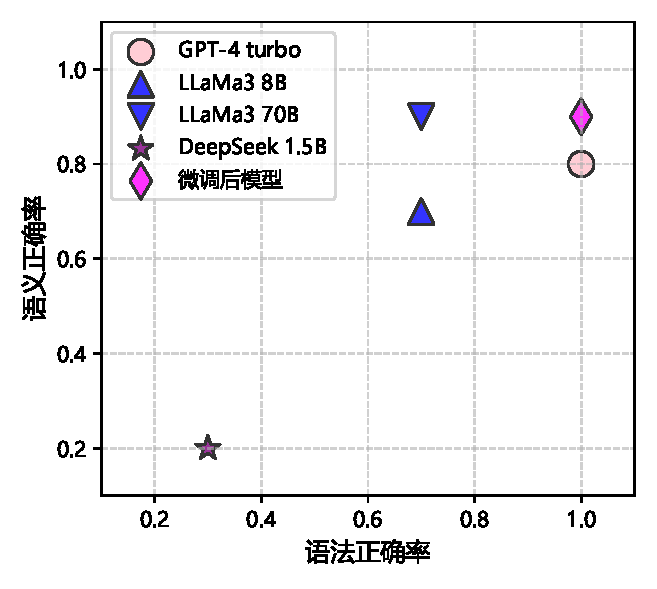
\includegraphics{figures/syntactics_and_semantics.pdf}
    \label{fig:syntactics_and_semantics}
    \caption{各模型的语法正确率及语义正确率}
\end{figure}
\begin{table}
    \centering
    \begin{tabular}{lcc}
        \toprule
        \textbf{模型} & \textbf{语法正确率} & \textbf{语义正确率} \\
        \midrule
        GPT-4 turbo & 1 & 0.8 \\
        Llama3 8B & 0.7 & 0.6 \\
        Llama3 70B & 0.7 & 0.8 \\
        DeepSeek R1 1.5B & 0.5 & 0.6 \\
        \midrule
        微调后模型 & 0.8 & 0.8 \\
        \bottomrule
    \end{tabular}
    \label{fig:overall_syntactics_semantics}
    \caption{各模型在语法和语义方面的对比分析}
\end{table}
\begin{table}[h]
    \centering
    \renewcommand{\arraystretch}{1.2}
    \setlength{\tabcolsep}{5pt}
    \resizebox{\textwidth}{!}{
    \begin{tabular}{lcccccccccccc}
        \toprule
        \multirow{2}{*}{模型} & \multicolumn{2}{c}{基础存在性} & \multicolumn{2}{c}{三维空间关系} & \multicolumn{2}{c}{多跳推理} & \multicolumn{2}{c}{多参考系} & \multicolumn{2}{c}{动态反事实} & \multicolumn{2}{c}{对抗性样本} \\
        \cmidrule(lr){2-3} \cmidrule(lr){4-5} \cmidrule(lr){6-7} \cmidrule(lr){8-9} \cmidrule(lr){10-11} \cmidrule(lr){12-13}
        & \textit{语法} & \textit{语义} & \textit{语法} & \textit{语义} & \textit{语法} & \textit{语义} & \textit{语法} & \textit{语义} & \textit{语法} & \textit{语义} & \textit{语法} & \textit{语义} \\
        \midrule
        GPT-4.0 turbo & 1 & 0.9 & 1 & 0.7 & 1 & 0.9 & 1 & 0.8 & 1 & 0.7 & 1 & 0.8 \\
        LLama3 8B & 0.9 & 0.6 & 0.7 & 0.5 & 0.8 & 0.6 & 0.6 & 0.7 & 0.5 & 0.7 & 0.7 & 0.5 \\
        LLama3 70B & 0.6 & 0.7 & 0.7 & 0.7 & 0.7 & 0.9 & 0.7 & 0.9 & 0.6 & 0.8 & 0.8 & 0.8 \\
        DeepSeek R1 1.5B & 0.5 & 0.6 & 0.7 & 0.5 & 0.6 & 0.6 & 0.4 & 0.7 & 0.4 & 0.5 & 0.5 & 0.7 \\
        \midrule
        \textbf{微调模型} & 1 & 0.9 & 0.8 & 1 & 0.6 & 0.9 & 0.9 & 0.8 & 0.9 & 0.8 & 0.6 & 0.4 \\
        \bottomrule
    \end{tabular}
    }
    \caption{不同模型在各问题类型上的语法正确率和语义正确率的对比}
    \label{tab:semantics_comparison}
\end{table}
\section{迭代反馈与规则修正}
迭代反馈模块是整个神经符号集成管道的核心部分,其主要功能在于提升由LLM生成的ASP程序的正确性和可执行性。
本文所提出的迭代反馈机制结合了自然语言解析、逻辑程序生成与符号求解三大过程,其整体流程可以描述为:
初步生成、逻辑程序执行、错误信息反馈、程序修正,直至达到预设的迭代次数或程序满足执行要求为止。
\subsection{反馈流程概述}
首先,LLM根据输入的自然语言描述生成初始的ASP程序,并将该程序交由Clingo求解器进行执行。
若在执行过程中出现任何错误(例如语法错误、变量命名不一致、或逻辑不严谨导致的求解失败),C
lingo将输出相应的错误信息。这些错误信息作为反馈被传递给LLM,指导其对初始生成的ASP程序进行针对性修正。
修正后的ASP程序再次输入Clingo求解器执行,如此循环最多进行三次,最终输出经过优化的ASP程序,
用于后续的正式推理。
\subsection{错误类型与修正策略}
不同类型的错误信息对应着ASP程序中不同的问题,因此需要采用不同的修正策略。
具体来说,本文设计了多套提示模板,用以指导LLM针对性地进行程序修正,其主要错误类型包括:
\begin{enumerate}
    \item 解析错误:如语法错误、未定义谓词、或不符合ASP语法要求的结构错误。针对该类错误,提示模板会明确指出错误的所在位置及其可能原因,并要求LLM调整相应的语法结构。
    \item 基础化错误:主要涉及变量命名不一致或不匹配等问题。此时,提示模板会强调变量的统一性和正确性,要求LLM对变量命名进行标准化处理。
    \item 求解阶段错误:包括过度约束或逻辑矛盾导致的求解失败。对于这类问题,提示模板将引导LLM重新审视程序中约束条件和规则之间的逻辑关系,并做出必要的修改。
\end{enumerate}
每一轮反馈过程中,LLM都将结合Clingo返回的错误信息和预定义的提示模板进行针对性修正,从而使生成的ASP程序在下一轮执行中更趋于正确和可执行。
\subsection{DSPy托管LLM调用}
为了高效管理这一LLM与ASP求解器之间的复杂的反馈交互过程,本文采用了DSPy框架。DSPy具备以下优势:
(1)模块化管理:DSPy将整个反馈流程拆分为若干功能模块,如ASP程序生成、错误信息解析、
提示模板更新及程序修正等。模块之间通过明确定义的接口进行通信,保证了信息的准确传递和记忆保留,
从而实现参数的自适应调整和流程优化。
(2)自动化优化:DSPy支持对LLM提示词及参数进行自动优化,极大地降低了人工调试的工作量。
在多次与LLM交互后,系统能够根据反馈动态调整提示模板,
最终得到一个较优的提示方案,以提高整体系统的修正效率和程序可执行率。
(3)日志记录与调试:为了便于调试和系统性能分析,
DSPy在整个反馈过程中对各模块的输出日志进行详细记录,包括错误信息、状态提示以及每一轮迭代的修正详情。
\subsection{DSPy优化器选择}
本文根据公开资料,对比了DSPy框架中提供的三种优化器的适用任务及场景,
如表\ref{tab:optimizer_comparison}所示。最终,本文选择了BootstrapFewShot优化器,其主要理由如下:
(1)标注成本低:传统的人工标注ASP事实需要较长时间(平均每个样本约3.5分钟),而BootstrapFewShot优化器针对少样本场景设计,仅需15-20个标注样本即可启动优化。
(2)分层次优化:BootstrapFewShot优化器将优化过程拆分为“教师优化”和“学生训练”两个阶段。教师优化阶段负责生成高质量的示例,而学生训练阶段则通过知识蒸馏完成对提示模板的优化,以确保整体修正效果的提升。
(3)资源控制:该优化器支持限制最大错误次数和迭代轮数,避免了无限循环和资源浪费,从而提高系统的稳定性与效率。

基于本文有限的标注样本和实际应用需求,选择BootstrapFewShot优化器能够在保证优化效果的同时,
大幅提高反馈迭代的效率和系统的总体性能。
\begin{table}[htbp]
\centering
\caption{Dspy 框架支持的优化器比较}
\label{tab:optimizer_comparison}
\begin{tabular}{|>{\raggedright}p{4cm}|>{\raggedright}p{8cm}|>{\raggedright\arraybackslash}p{4cm}|}
\hline
\textbf{优化器名称} & \textbf{主要功能} & \textbf{适用场景} \\
\hline
BootstrapFewShot & 通过在提示中自动生成并包含优化示例来扩展签名。 & 少样本学习 \\
\hline
BootstrapFewShot-
WithRandomSearch & 在 BootstrapFewShot 的基础上,对生成的示例进行多次随机搜索,选择优化后的最佳程序。 & 少样本学习,需要更高精度 \\
\hline
MIPRO & 在每个步骤中生成指令和少量示例,使用贝叶斯优化来有效地搜索模块中的生成指令和示例空间。 & 需要复杂指令和示例优化的场景 \\
\hline
BootstrapFinetune & 将基于提示的 DSPy 程序提炼为较小语言模型的权重更新,微调底层大型语言模型以提高效率。 & 需要微调模型以提高效率的场景 \\
\hline
\end{tabular}
\end{table}
\section{规则蒸馏}
经过迭代反馈修正后的ASP编码,已经能够顺利通过Clingo求解器执行,同时在语法和语义上保证正确。然而,要正确进行推理,
可能还需要先验知识配合。规则蒸馏的目的在于,利用LLM的知识和已有ASP知识库的知识,对迭代反馈修正后得到的
ASP编码进行补全,减轻知识工程师手动编写规则的负担,最终得到解决问题所需的足够的ASP规则,供后续Clingo求解器
使用。

本模块的技术路径如下:
当系统检测到现有的ASP规则集无法推导出问题的正确答案时,将会
\subsection{预提示}
预提示的作用是,为LLM提供背景信息和任务说明。具体而言,预提示包括以下内容:(1)任务背景说明。介绍
VQA任务场景,说明问题和图像已经被解析为ASP表示;(2)ASP语法与表示。讲解ASP的语法以及如何使用ASP表示
场景、问题和答案,使LLM了解输入格式;(3)初始理论。给LLM提供ASP规则,这些规则来源于本地的ASP知识库;
(4)任务要求。明确向LLM要求,输出内容不仅包括新规则的ASP代码,并且要求规则尽可能通用,不应包含具体事实。

该机制通过增量式规则扩展实现ASP知识库的动态演进:每当系统识别出现有理论无法推导正确结果时,
会触发LLM的规则生成模块,输出符合ASP语法的逻辑规则补充到ASP知识库中。
整个过程形成"问题识别-规则生成-理论扩展"的闭环优化路径。

以下为节选的部分提示词。
\begin{lstlisting}
你的任务是对ASP知识库进行维护,通过动态更新规则确保其能够解答各类问题。ASP知识库中的现有规则已能够满足对部分问题的处理需要,
需根据输入的问题的ASP表示进行增量式规则拓展。输入提示将包含一个或多个采用ASP表示形式的问题。请严格遵守以下规则:

1. 仅输出新增的ASP规则。
2. 禁止将事实作为规则添加。不允许在规则头(head)中使用具体常量实例。
3. 将规则的泛化程度实现最大化。你输出的规则应具备以下特征:使用大写字母变量(如X,Y,Z)替代具体常量,通过谓词逻辑建立抽象关系而非具体实例关联。
4. 完全禁用自然语言。你的输出中,不得出现任何自然语言成分,包括:错误提示信息、代码注释说和解释性文字。
\end{lstlisting}
\subsection{规则蒸馏算法}
向LLM进行预提示之后,对迭代反馈后的ASP代码和视觉场景理解模块得到的ASP代码,合并记作$p$,执行如下步骤(最多重复$r$次):

\begin{enumerate}[itemsep=0pt,parsep=0pt]
    \item 提示。将$p$作为附加输入提示LLM,并得到响应$R$。
    \item 求解。将响应$R$与ASP知识库中的初始知识$I$结合,得到新的ASP规则集$Res$。基于$Res$,调用Clingo求解器
对问题进行求解。此后首先进行语法检查,若检测到语法错误,则将错误信息传给LLM,并要求$R$进行修改,最多重试$m$次。
此外进行语义检查,验证求解器的输出是否与预期答案一致,如果不一致则将实际答案和预期答案传给LLM,要求其对$R$进行更新,最多重试$m$次。
    \item 回归测试。为了避免新增加的规则破坏知识库中规则的一致性,需要对$Res$进行测试。只有当所有的
测试都通过之后,才会保留$Res$,否则将会忽略$R$。
\end{enumerate}

以上算法有2个参数,$r$是每个示例的重试次数,$m$是修正错误规则的重试次数。$r$和$m$的默认值都为1。

为了对规则蒸馏LLM进行训练,补充ASP知识库,在此处采用了GQA数据集以拓展现有的ASP知识库。对GQA数据集中的
问答数据进行预处理后,每条数据均以(问题,场景,答案)的三元组形式给出,数据集中的实例被用来检测当前ASP理论的不足,
并引导LLM生成补充规则,以便在语法和语义检查通过后将新规则融入系统中,从而提升整体推理能力。 
\section{ASP推理}
ASP推理阶段中,ASP求解器接收经过优化后的ASP查询语句、视觉场景理解模块提取的ASP事实以及已有常识的ASP表示,进行逻辑推理,最终获得答案。
本文使用Clingo求解器来进行求解,其工作过程分为基础化(grounding)阶段和求解(solving)阶段。

基础化阶段将ASP程序中的变量替换为常量,生成一个新的ASP程序。Clingo
通过使用内置的基础化器分析程序,生成所有可能的规则。例如,对规则
$a(X) :- b(X), not c(X).$,其将被展开为所有可能的值为X的实例。

求解阶段中,Clingo采用类似SAT求解器的冲突驱动答案集求解(CDNL)方法。CDNL方法通过迭代地添加约束,直到找到一个满足所有约束的解,或者证明无解。
具体而言,Clingo基于如下步骤进行求解:(1)初始化。从空分配开始(没有原子被标记为真);
(2)选择与分配。选择一个未分配的原子,猜测其真值为真或假;
(3)传播。根据当前分配和规则,推导其他原子的真值。例如,若规则$a :- b, not c.$满足,b为真且c不在答案集中,则a必须为真;
(4)冲突检测。若分配导致规则冲突(如与已有的约束条件相抵触),记录冲突原因;
(5)回溯与学习。若发生冲突,回溯到之前的选择点,学习冲突子句以避免未来类似错误;
(6)验证。当所有原子分配完成后,检查是否为答案集,即确保它是程序的模型,且最小化(无子集也能满足规则)。

相比其它的ASP求解器,Clingo在以下几个方面进行了优化:(1)从冲突中学习
新的规则,为将来进一步的搜索提供指导;(2)使用多线程实现并行化,同时搜索
多个路径,加速求解过程;(3)使用启发式方法决定分配顺序,例如优先选择高影响力的原子;
(4)预测可能发生的冲突,选择可能导致冲突的原子优先分配,减少搜索空间。
\section{求解结果翻译}
经过Clingo得到的输出结果,以ASP谓词表示,对用户而言并不友好。需要将其转为自然语言。
Clingo输出的是由逻辑谓词构成的答案集,例如谓词\textbf{is(A, left, B)}表示“A位于B的左侧”。
由于正常情况下,Clingo输出的都是预定义的谓词,故采用构造同义词字典的方案,将ASP中的逻辑谓词与自然语言
表述对应起来。LLM可基于这些模板对解析后的逻辑结果进行填充和修正,生成标准化且易于理解的描述。
\section{实验与结果分析}
\subsection{对比试验}
为全面评估神经符号框架的有效性以及泛化能力,本文选取了目前主流的三种LLM:DeepSeek R1、
Llama3和GPT-4 turbo,在其上应用神经符号框架,进行对比。以上既包含DeepSeek这类轻量级专用模型,
也涵盖GPT-4 turbo这类通用型先进系统,而Llama3性能和效率之间取得了平衡,属于居中水平的模型。通过
在多个基座上进行实验,证明神经符号框架对不同LLM的泛化能力。

基线模型一选取直接提示VLM的方式,即直接将自然语言问题和图像输入到VLM中,并不给予任何的额外提示。
直接提示VLM的方式虽然简单,却是评估模型的关键基准,因为直接提示方法能够反映模型在没有任何
外部推理辅助机制的情况下,自身对空间问题的处理能力。

基线模型二采用“事实+规则”的提示方法。该方法的核心思路是:指示LLM使用预先定义的谓词,将输入的自然语言问题转换为结构化事实,然后LLM应用相关逻辑
规则,通过自然语言推理答案。
“事实+规则”的提示方法满足了将原始自然语言问题转为结构化符号表示,以配合视觉场景理解所得的ASP事实以及原有常识,共同进行推理的核心需求。同时,
该方法使用具有精确参数结构的谓词对LLM进行提示,使得LLM可以创建一致的中间态的知识表示,为问题解答提供便利。综合来看,“事实+规则”的提示方法作为一种
简化流程,既保留了形式化推理的优势,同时能够避免在生成ASP程序时和LLM进行多次交互,进而降低对计算资源的要求,降低了成本,也减少了对外部求解器的依赖。

实验结果见表\ref{tab:overall_comparison},本文提出的神经符号框架在DeepSeek R1、LLama3和GPT-4.0 turbo上均超过了两种比较基准方法,证明大语言模型与逻辑推理结合对于解决
复杂空间推理问题的有效性。

\begin{table}[h]
    \centering
    \small  % 调整字体大小(可选:\footnotesize 更紧凑)
    \renewcommand{\arraystretch}{1.2}  % 增加行距
    \setlength{\tabcolsep}{5pt}  % 调整列间距
    \resizebox{\textwidth}{!}{  % 让表格自适应页面宽度
    \begin{tabular}{lcccccc}
        \toprule
        \textbf{模型及方法} & \textbf{基础存在性问题} & \textbf{三维空间关系问题} & \textbf{多跳推理问题} & \textbf{多参考系问题} & \textbf{对抗性样本问题} & \textbf{总体} \\
        \midrule
        \multicolumn{7}{c}{\textbf{DeepSeek R1}} \\  
        直接提问 & 60.5 & 38.2 & 74.5 & 78.2 & 48.2 & 59.9 \\
        事实+规则提示方法 & 69.7 & 47.3 & 80.6 & 80.9 & 56.6 & 67.0 \\
        神经符号框架方法 & 77.8 & 58.9 & 85.4 & 81.8 & 42.8 & 69.3 \\
        \midrule
        \multicolumn{7}{c}{\textbf{Llama3}} \\  
        直接提问 & 68.4 & 26.9 & 65.7 & 72.5 & 55.8 & 57.9 \\
        事实+规则提示方法 & 75.3 & 46.8 & 70.2 & 81.4 & 57.1 & 66.2 \\
        神经符号框架方法 & 79.1 & 53.1 & 83.3 & 80.5 & 60.8 & 71.4 \\
        \midrule
        \multicolumn{7}{c}{\textbf{GPT-4.0 turbo}} \\  
        直接提问 & 77.2 & 45.4 & 60.9 & 57.6 & 58.2 & 59.9 \\
        事实+规则提示方法 & 85.3 & 54.3 & 68.2 &61.5 & 50.4 & 64.0 \\
        神经符号框架方法 & 91.1 & 65.6 & 80.5 & 72.7 & 64.8 & 74.9 \\
        \bottomrule
    \end{tabular}
    }
    \caption{不同模型及方法在各问题类型上的表现}
    \label{tab:overall_comparison}
\end{table}

\subsection{消融实验}
尽管LLM在语义解析任务中表现出色,但其生成的ASP程序的正确率仍有较大的提升空间。Feng\cite{feng2024language}等人的研究表明,将自然语言直接转为逻辑规则的
成功率一般较低。而神经符号框架通过在LLM和外部ASP求解器之间设立反馈循环机制,使LLM能够根据ASP求解器在试图求解ASP程序之前的语法检查结果,对生成的ASP程序
中的错误进行修正,极大提高了将自然语言问题转为ASP程序的准确率。

为进一步探讨神经符号框架的迭代反馈机制的作用,本文重点关注ASP求解器执行过程中常发生的三类主要错误:解析错误、实例化失败以及求解阶段失败。
另外,即便生成的ASP程序执行成功,也有很大可能由于自然语言问题与LLM生成的ASP程序之间不一致,而产生与真实答案偏离的结果。

在测试中,迭代反馈机制显著提升了所有模型的性能。如图\ref{fig:ablation}所示,经过两轮迭代反馈之后,DeepSeek R1的可执行率从51.3\%提升到了84.2\%,LLama3的可执行率从60.2\%提升到了89.7\%
,GPT-4.0 turbo的可执行率从64.6\%提升到了91.1\%。
在准确率方面,DeepSeek R1的准确率从57.8\%提升到了79.3\%,LLama3的准确率从61.1\%提升到了85.7\%,GPT-4.0 turbo的准确率从69.7\%提升到了93.4\%。
以上结果表明,LLM与ASP求解器之间的迭代反馈机制能有效解决自然语言到逻辑程序的转换过程中面临的问题。对准确率和可执行率的提升,主要集中在
第一轮迭代反馈中,此后继续迭代的效果呈现边际递减趋势。由于计算资源有限,本次消融实验仅进行了三轮。实验结果有力证明,迭代反馈机制在提升ASP程序的可执行率和
正确率方面具有明显效果,充分验证了神经符号方法的有效性。

\begin{figure}
    \centering
    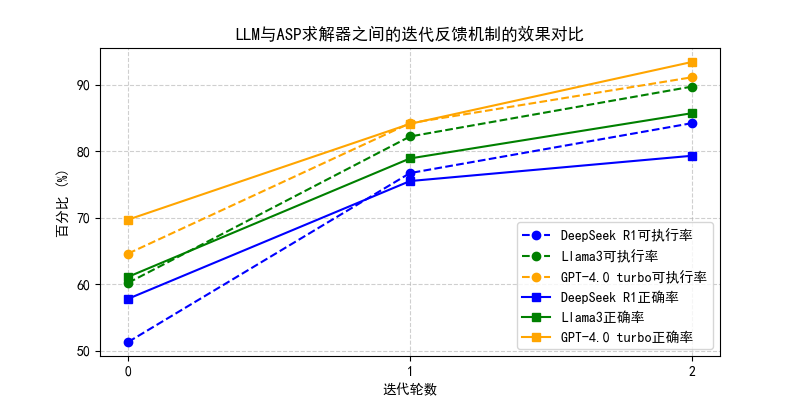
\includegraphics[width=\textwidth]{ablation.png}
    \caption{LLM与ASP求解器之间的迭代反馈机制的效果对比}
    \label{fig:ablation}
\end{figure}

\section{本章小结}
本章详细介绍了神经符号框架的整体架构设计与实现过程,阐述了从视觉场景理解、语义解析、迭代反馈与规则修正
到规则蒸馏,
再到最终的ASP推理的完整流水线。首先,框架总体架构明确了LLM在语义解析和反馈优化中的双重作用,
为复杂空间关系推理提供了有效支撑。接着,在视觉场景理解部分,本文基于GLIP模型实现了目标检测,
并通过中心点与深度信息提取物体的二维及三维位置信息,再结合空间关系提取技术构建场景图,
并将提取的信息转化为ASP事实,为后续逻辑推理打下坚实基础。

在语义解析模块中,利用LLM的上下文学习能力,通过微调生成与自然语言问题对应的ASP程序,
设计了多种ASP模板以覆盖基础存在性、三维空间关系、多跳推理、多参考系、动态反事实以及对抗性样本等问题类型。
实验结果表明,经过微调和DSPy框架支持下的提示优化,生成的ASP查询在语法与语义上均取得了较高准确率,
验证了LLM在语义解析任务中的有效性。

随后,通过迭代反馈与规则修正模块,系统实现了LLM与ASP求解器之间的闭环交互:
Clingo求解器对生成的ASP程序进行执行检查,并反馈错误信息,LLM据此优化ASP程序,
经过多轮迭代后显著提升了程序的可执行率和语义正确率。接着,通过规则蒸馏模块,以迭代反馈与规则修正模块得到
的ASP代码和视觉场景理解得到的ASP代码为输入,以ASP知识库为基础,调用LLM对ASP规则进行补充,同时对ASP知识库进行
更新完善。
最后,在对比试验和消融实验中,
本文综合比较了不同LLM模型和提示方法的表现,验证了神经符号框架在处理复杂空间推理问题上的泛化能力与优势,
同时也证明了迭代反馈机制对整体性能提升的重要作用。

总体来说,本章不仅构建了一个完整而高效的神经符号推理流水线,而且通过详细实验与消融分析,
验证了各模块间协同工作的有效性,为后续基于逻辑推理的VQA系统提供了坚实的理论和实践基础。